\usepackage[noblocks]{authblk}
\renewcommand*{\Authsep}{, }
\renewcommand*{\Authand}{, }
\renewcommand*{\Authands}{, }
\renewcommand\Affilfont{\small}
\usepackage{amssymb}
\usepackage{booktabs} % Add to your preamble for cleaner table lines
\usepackage{makecell} % Add to your preamble for multi-line cells
\usepackage{tikz}
\usepackage{amsmath}
\usetikzlibrary{arrows.meta, shapes.geometric}

%% Define TikZ arrow styles
\newcommand{\starstar}{% 
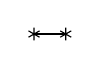
\begin{tikzpicture}[baseline=-3pt]
    \draw [{Rays[n=6]}-{Rays[n=6]}] (0,0) -- (0.55,0);
\end{tikzpicture}
}

\newcommand{\circstar}{% 
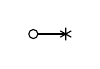
\begin{tikzpicture}
    \draw [{Circle[open]}-{Rays[n=6]}] (0,0) -- (0.55, 0);
\end{tikzpicture}
}

\newcommand{\starcirc}{% 
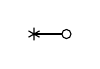
\begin{tikzpicture}
    \draw [{Rays[n=6]}-{Circle[open]}] (0,0) -- (0.55, 0);
\end{tikzpicture}
}

\newcommand{\stararrow}{% 
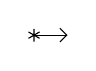
\begin{tikzpicture}
    \draw [{Rays[n=6]}-{Straight Barb[length=2.5pt]}] (0,0) -- (0.5, 0);
\end{tikzpicture}
}

\newcommand{\arrowstar}{% 
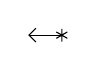
\begin{tikzpicture}
    \draw [{Straight Barb[length=2.5pt]}-{Rays[n=6]}] (0,0) -- (0.5, 0);
\end{tikzpicture}
}

\newcommand{\circarrow}{% 
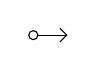
\begin{tikzpicture}
    \draw [{Circle[open]}-{Straight Barb[length=2.5pt]}] (0,0) -- (0.5, 0);
\end{tikzpicture}
}

\newcommand{\tailcirc}{% 
\begin{tikzpicture}[baseline=-3pt] 
    \draw [-{Circle[open]}] (0,0) -- (0.4, 0);
\end{tikzpicture}
}

\newcommand{\circtail}{% 
\begin{tikzpicture}[baseline=-3pt] 
    \draw [{Circle[open]}-] (0,0) -- (0.4, 0);
\end{tikzpicture}
}

\newcommand{\circirc}{% 
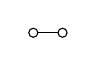
\begin{tikzpicture}[baseline=-3pt] 
    \draw [{Circle[open]}-{Circle[open]}] (0,0) -- (0.5, 0);
\end{tikzpicture}
}

\newcommand{\tailstar}{% 
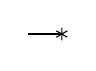
\begin{tikzpicture}[baseline=-3pt] 
    \draw [-{Rays[n=6]}] (0,0) -- (0.5, 0);
\end{tikzpicture}
}

\newcommand{\startail}{% 
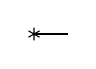
\begin{tikzpicture}
    \draw [{Rays[n=6]}-] (0,0) -- (0.5, 0);
\end{tikzpicture}
}

\newcommand{\tailarrow}{% 
\begin{tikzpicture}
    \draw [-{Straight Barb[length=2.5pt]}](0,0) -- (0.4, 0);
\end{tikzpicture}
}

\newcommand{\arrowtail}{% 
\begin{tikzpicture}
    \draw [{Straight Barb[length=2.5pt]}-](0,0) -- (0.4, 0);
\end{tikzpicture}
}

\newcommand{\arrowarrow}{% 
\begin{tikzpicture}
    \draw [{Straight Barb[length=2.5pt]}-{Straight Barb[length=2.5pt]}](0,0) -- (0.4, 0);
\end{tikzpicture}
}

\newcommand\stackedarrows{%
        \mathrel{\vcenter{\mathsurround0pt
                \ialign{##\crcr
                \noalign{\nointerlineskip}$\arrowtail$\crcr
                \noalign{\nointerlineskip}$\tailarrow$\crcr
                }
        }}%
}